\documentclass[journal]{IEEEtran}

\usepackage{amsmath}
\usepackage{amssymb}
\usepackage{graphicx}
\usepackage{booktabs}
\usepackage[hidelinks]{hyperref}

\begin{document}

\title{Safe-Escape MPPI: Coordinating Online Local-Minima Escape with\\
Control-Barrier-Function Safety in a Nav2-Native Controller}

\author{Jung~Mo~Kang% <-this % stops a space
\thanks{J.~M.~Kang is an independent researcher based in
Seoul, Republic of Korea (e-mail: kangjmo91@gmail.com).}}

\markboth{Preprint submitted to IEEE Robotics and Automation Letters (RA-L)}%
{Kang: Safe-Escape MPPI}

\maketitle

\begin{abstract}
The Model Predictive Path Integral (MPPI) controller shipped with ROS~2
Nav2 is among the strongest deployable local controllers for mobile robots,
yet in narrow, crowded, dynamic spaces it is prone to local-minima
entrapment and enforces collision avoidance only through soft costs, with
no formal safety guarantee. Prior work treats these weaknesses in
isolation, and none ships as a deployable Nav2 controller. We present
Safe-Escape MPPI (SE-MPPI), a single Nav2-native controller that unifies
online local-minima detection-and-escape with a dynamic-obstacle
control-barrier-function (CBF) safety filter, reconciled by a coordinator
that modulates the barrier's class-$\mathcal{K}$ gain on detected
entrapment. Forward invariance is preserved for any positive gain, so an
escape maneuver admitted by a raised gain stays certified-safe. In a randomized $1{,}200$-trial 2D benchmark
mirroring the controller math one-to-one, the detection-and-escape layer
is the decisive contribution on both trap families, with the free-space
gap search load-bearing. The escape--safety coordination instead matches an
independent escape+CBF stack -- a null result: outcomes are insensitive to
the barrier-gain schedule even where the barrier engages -- so we claim it
as a certified-safe mechanism, not an empirical gain. The controller also
runs inside a live ROS~2 Jazzy + Nav2 + Gazebo stack, and we report the
deployment faults live integration exposes.
\end{abstract}

\begin{IEEEkeywords}
Model predictive control, control barrier functions, collision avoidance,
local-minima escape, motion and path planning, autonomous navigation,
ROS~2 Nav2.
\end{IEEEkeywords}

\section{Introduction}
\label{sec:intro}

Autonomous mobile robots increasingly operate in cluttered, dynamic indoor
environments -- warehouses, hospitals, service floors -- where the local
controller must be simultaneously \emph{fast}, \emph{non-conservative}, and
\emph{safe}. Within the ROS~2 Nav2 ecosystem, the MPPI controller
(\texttt{nav2\_mppi\_controller}) \cite{nav2} has become the de-facto
high-performance choice: it supports differential, omnidirectional, and
Ackermann robots and runs at 50+~Hz on CPU by sampling \texttt{batch\_size}
rollouts, scoring them with a bank of critics, and combining them with an
information-theoretic softmax \cite{mppi_orig}.

Two weaknesses, however, recur exactly in the environments that matter
most:

\begin{enumerate}
\item \textbf{Local-minima entrapment.} A finite prediction horizon (by
  default $56 \times 0.05\,\mathrm{s} \approx 2.8\,\mathrm{s}$) and
  zero-mean Gaussian sampling cause the robot to stall or oscillate in
  non-convex traps. Nav2's only mitigations are \emph{always-on}
  cost-shaping heuristics (\texttt{PreferForwardCritic},
  \texttt{TwirlingCritic}) that neither \emph{detect} entrapment nor
  guarantee escape.
\item \textbf{No formal safety.} Avoidance is encoded as soft costs
  (\texttt{ObstaclesCritic}, \texttt{CostCritic}); there is no
  forward-invariance guarantee, and crucially \textbf{no prediction of
  dynamic-obstacle motion} -- the costmap is a present-time snapshot and
  \texttt{collision\_monitor} is purely reactive.
\end{enumerate}

These weaknesses interact: being conservative for safety invites
entrapment, and escaping aggressively invites collision. We argue they
should be solved \emph{together}, in one deployable controller.
Fig.~\ref{fig:mechanism_panels}(a) (Sec.~\ref{sec:mechanism}) illustrates
the first weakness and SE-MPPI's response: stock MPPI stalls before a U-shaped
trap while SE-MPPI detects the entrapment and rounds it under the
certified-safe coordination of Sec.~\ref{sec:coordination}.

\textbf{Contributions.}
\begin{itemize}
\item \textbf{C1 (system).} To our knowledge, the first
  \textbf{Nav2-native local controller plugin} that combines a CBF safety
  filter with online local-minima escape; packaged as a
  \texttt{nav2\_core::Controller} plus a pluginlib MPPI critic.
\item \textbf{C2 (algorithm).} An \textbf{escape--safety coordination}
  mechanism that modulates the CBF class-$\mathcal{K}$ gain on detected
  entrapment, letting the robot escape \emph{without} losing forward
  invariance (proven in Sec.~\ref{sec:coordination}), with a TTC override
  that re-prioritizes safety when a dynamic obstacle's time-to-collision is
  imminent. We claim C2 as a certified-safe \emph{mechanism}: in our 2D
  benchmark it is empirically indistinguishable from an independent
  escape+CBF stack (Sec.~\ref{sec:evsf}) -- outcomes proved insensitive to
  the barrier-gain schedule even where the barrier engages.
\item \textbf{C3 (dynamic safety).} Integration of a look-ahead-point CBF
  safety filter for a differential-drive robot, fed by a costmap-based
  dynamic-obstacle tracker, as a QP at the controller's output.
\item \textbf{C4 (reproducibility).} An open Apache-2.0
  implementation,\footnote{Code, benchmark scripts, and raw trial data:
  \url{https://github.com/kjungmo/se-mppi-nav2} (Apache-2.0); see the
  Appendix for the regeneration commands.} a
  standalone 2D mechanism validation, a randomized $1{,}200$-trial 2D
  benchmark with paired significance tests, and a specified full-scale
  ROS~2 physics-benchmark protocol.
\end{itemize}

We are deliberately conservative about novelty and about what we claim
empirically: fusing CBFs with MPPI is \emph{not} new. Our measured win is
the online detection-and-escape layer ($0\%\!\to\!88$--$90\%$ on the static
U-trap family, Holm-adjusted $p=1.4\times10^{-9}$, and
$0\%\!\to\!62$--$78\%$ on the narrow-dynamic family,
$p_\text{adj}=1.1\times10^{-6}$, with
the gap search load-bearing; Sec.~\ref{sec:bench2d}). The
escape--safety coordination (C2) is a certified-safe mechanism
(Sec.~\ref{sec:coordination}) that, in the regime we could test, is
empirically indistinguishable from an independent escape+CBF stack; we
report this null openly and delimit where coordination should matter. The
remaining load-bearing claims are Nav2-native deployment and the deployment
faults a live stack exposes.

\section{Related Work}
\label{sec:related}

\textbf{MPPI and local controllers.} Nav2 MPPI \cite{nav2,mppi_orig}, TEB
\cite{teb}, DWB (a Nav2 DWA-family planner) \cite{dwa}, and Regulated Pure
Pursuit \cite{rpp} are the standard deployable local planners. MPPI's
critic-plugin interface (\texttt{mppi::critics::CriticFunction}) exposes
per-rollout trajectories, the reference path, the goal, collision flags,
and the furthest-reached path index -- i.e., the signals needed for
entrapment detection are already available, and a custom critic can be
inserted without forking the optimizer.

\textbf{Local-minima escape.} Most methods are \emph{always-on}
augmentations of the sampling distribution: log-MPPI \cite{log_mppi},
Tsallis-MPPI \cite{tsallis_mppi}, SVG-MPPI (Stein mode-seeking)
\cite{svg_mppi}, Biased-MPPI \cite{biased_mppi}, and learned sampling
distributions for MPC (Sacks and Boots) \cite{flow_mppi}. The closest
prior \emph{detect-and-switch} method is \textbf{DRPA-MPPI} (Fuke et~al.,
2025 preprint) \cite{drpa_mppi}, which detects entrapment from predicted
trajectories and
switches on a repulsive-potential cost. DRPA-MPPI has no CBF or formal
safety, models no dynamic obstacles, ships no public code, and is not
Nav2-integrated. SE-MPPI uses it as the escape baseline.

\textbf{CBF~$\times$~MPPI safety.} All four fusion styles exist as
research code: soft cost/critic (Shield-MPPI \cite{shield_mppi}, BR-MPPI
\cite{br_mppi}), output QP filter (CBFKit \cite{cbfkit}, the Shield
stage), unsafe-sample rejection (reach-avoid SCBF-MPPI \cite{scbf_mppi},
DualGuard stage~1 \cite{dualguard}), and provably-safe
projection/shielding (GS-MPPI \cite{gs_mppi}, DualGuard
\cite{dualguard}). For dynamic obstacles, DPCBF (``Beyond Collision
Cones,'' ICRA 2026) \cite{dpcbf} uses a parabolic safe set that is far
less conservative than collision-cone/velocity-obstacle CBFs and stays
QP-feasible in dense dynamic scenes -- but is QP-only and not embedded in
MPPI. Critically, \emph{none of these ship as a Nav2 controller} (CBFKit
builds a standalone node).

\textbf{Conformal prediction for safe control (background, not claimed).}
The released controller carries an online conformal margin that inflates
the CBF effective radius under prediction uncertainty; this is an
implementation detail deferred to follow-up work
(Sec.~\ref{sec:limitations}, SE-Predict) and is \emph{not} a contribution of
this paper. That margin draws on the established line of
conformal-prediction-for-safe-control work
\cite{acp_yang,conformal_hri,lindemann,dixit,ua_pcbf}; Paper~1's claims are
C1--C4 and stand without it.

\textbf{Positioning.} SE-MPPI occupies a four-way intersection that no
single prior work holds, based on a June 2026 review of the Nav2-MPPI critic
ecosystem, the CBF--MPPI fusion papers cited above, and the ROS Discourse /
GitHub issue threads for these projects: \textbf{(a)}~a Nav2-native plugin,
\textbf{(b)}~online local-minima escape, \textbf{(c)}~a dynamic-obstacle CBF
safety filter, and \textbf{(d)}~escape--safety gain coordination.
Table~\ref{tab:positioning} tabulates the named systems against these four
factors: no reviewed work holds more than one, and in particular no
Nav2-native controller carries a CBF. Element (d) -- the gain coordination
-- is the cleanest unoccupied contribution.

\begin{table}[t]
\centering
\caption{Positioning against factors \textbf{(a)}~Nav2-native plugin,
\textbf{(b)}~online local-minima escape, \textbf{(c)}~dynamic-obstacle CBF
safety filter, \textbf{(d)}~escape--safety gain coordination. No reviewed
prior system holds more than one; SE-MPPI is the only work at the
four-way intersection.}
\label{tab:positioning}
\footnotesize
\setlength{\tabcolsep}{5pt}
\begin{tabular}{lcccc}
\toprule
System & (a) & (b) & (c) & (d) \\
\midrule
DRPA-MPPI \cite{drpa_mppi}                        & --         & \checkmark & --         & --         \\
Shield-/BR-MPPI \cite{shield_mppi,br_mppi}        & --         & --         & \checkmark & --         \\
CBFKit \cite{cbfkit}                              & --         & --         & \checkmark & --         \\
SCBF-MPPI / DualGuard \cite{scbf_mppi,dualguard}  & --         & --         & \checkmark & --         \\
GS-MPPI \cite{gs_mppi}                            & --         & --         & \checkmark & --         \\
DPCBF \cite{dpcbf}                                & --         & --         & \checkmark & --         \\
\textbf{SE-MPPI (ours)}                           & \checkmark & \checkmark & \checkmark & \checkmark \\
\bottomrule
\end{tabular}
\end{table}

\section{Problem Formulation}
\label{sec:problem}

Consider a differential-drive robot with pose $(x,y,\theta)$ and control
$u=(v,\omega)$, tracking a global path $\sigma$ produced by a Nav2 global
planner, amid static structure and a set $\mathcal{O}$ of dynamic
obstacles $o$ with position $p_o$, radius $R_o$, and (estimated) velocity
$v_o$. Let $r$ be the robot's inscribed radius and $m$ a safety margin. We
want a control policy that (G1)~makes monotone progress along $\sigma$ --
i.e., does not stall in a local minimum -- and (G2)~keeps the robot
collision-free with respect to $\mathcal{O}$ with a forward-invariance
guarantee, while (G3)~running as a Nav2 controller at $\geq 10$~Hz on CPU.

The tension: G1 may require maneuvers that approach obstacles (to round a
trap), whereas a naive safety filter for G2 forbids exactly those
maneuvers. SE-MPPI's coordinator (Sec.~\ref{sec:coordination}) is the
mechanism that satisfies G1 and G2 jointly.

\section{Method: SE-MPPI}
\label{sec:method}

\subsection{Overview}
\label{sec:overview}

SE-MPPI subclasses the stock \texttt{MPPIController}, reusing its
optimizer for the nominal command, then post-processes that command each
cycle:

\begin{enumerate}
\item \textbf{Entrapment detection} from monotone global-path progress
  (single source of truth, shared with the critic).
\item \textbf{Escape} at sampling time: an \texttt{EscapeCritic} injects
  distance-field APF and free-space gap-attraction costs \emph{only when
  entrapment is detected}.
\item \textbf{Dynamic-obstacle tracking} from the local costmap.
\item \textbf{Coordination}: resolve the CBF gain $\alpha$ from
  entrapment and TTC.
\item \textbf{CBF safety filter}: project the nominal $(v,\omega)$ onto
  the CBF-safe set via a small QP.
\end{enumerate}

The escape and safety layers thus act at complementary points --
sampling-time cost shaping and output-time projection -- unified by a
shared entrapment signal and the coordinated gain.

\begin{figure*}[t]
\centering
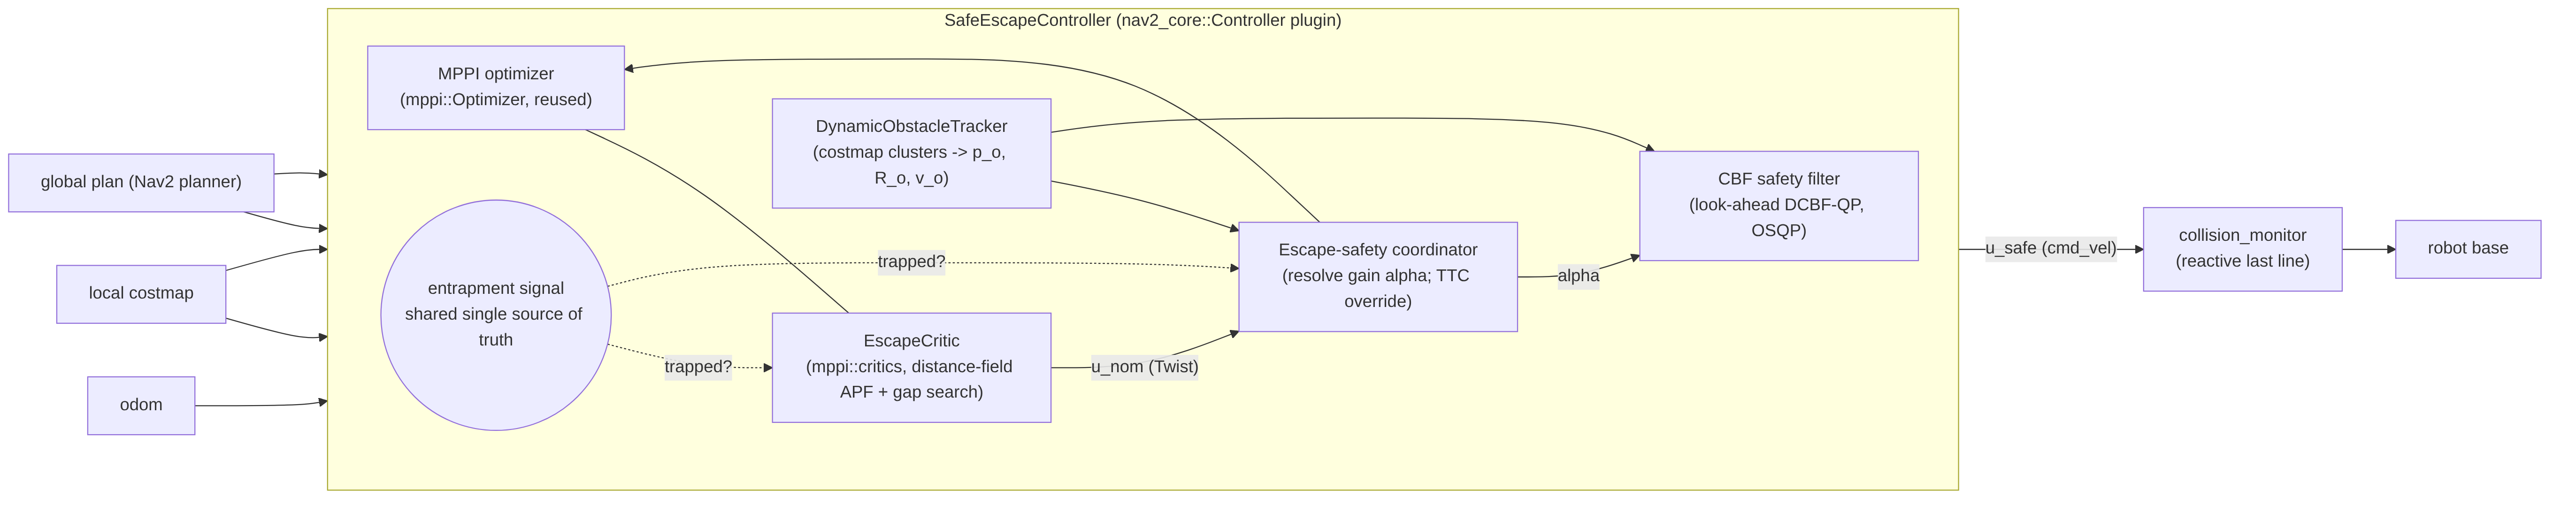
\includegraphics[width=0.85\textwidth]{figures/architecture.png}
\caption{SE-MPPI architecture / data flow. Global plan, local costmap, and
odometry feed the \texttt{SafeEscapeController} plugin: the reused MPPI
optimizer (with the \texttt{EscapeCritic}) emits the nominal command, a
shared entrapment signal drives both the critic and the escape--safety
coordinator, the coordinator resolves the CBF gain $\alpha$ (with TTC
override), and the CBF safety filter -- fed by the
\texttt{DynamicObstacleTracker} -- projects the command to
\texttt{cmd\_vel}, which Nav2's \texttt{collision\_monitor} guards as a
final reactive layer.}
\label{fig:architecture}
\end{figure*}

Fig.~\ref{fig:architecture} summarizes the resulting data flow.

\subsection{Entrapment detection (single source of truth)}
\label{sec:entrapment}

\texttt{nearestPathIndex}$(\sigma)$ is non-monotone, so we track the
\textbf{furthest reached} path index $k_{\max}$ and declare entrapment
when $k_{\max}$ fails to advance for a window of $W$ cycles (default 30;
the 2D benchmark of Sec.~\ref{sec:bench2d} uses 15). Entrapment is suppressed within a goal tolerance so a robot
finishing at the path end does not trigger a false escape. The controller
is the \emph{only} detector; the \texttt{EscapeCritic} and the coordinator
read the same shared atomic state via a registry keyed by the controller
name, so escape and safety always agree on whether the robot is trapped.

\subsection{Escape (detect-and-switch)}
\label{sec:escape}

On entrapment the \texttt{EscapeCritic} adds two cost terms to the MPPI
rollouts:
\begin{itemize}
\item \textbf{Distance-field APF}
  $U=\tfrac12\eta\,(1/d - 1/d_0)^2$ for $d<d_0$, where $d$ is the Dijkstra
  distance to the nearest obstacle cell (excluding unknown space), which
  pushes rollouts off the trapping surface; and
\item \textbf{Free-space gap attraction}: a ray-cast around the robot
  finds the opening whose bearing is closest to the goal direction and
  whose clearance exceeds a threshold, and rollouts heading toward that
  gap are rewarded -- providing a temporary subgoal that rounds
  non-convex (U-shaped) traps.
\end{itemize}

Because the terms are injected only when entrapped, free-space behavior is
unchanged (detect-and-switch, not always-on).

\subsection{CBF safety filter (dynamic obstacles)}
\label{sec:cbf}

To make the barrier relative-degree one in $(v,\omega)$ for a unicycle,
safety is enforced on a \textbf{look-ahead point}
$P = (x,y) + L\,(\cos\theta,\sin\theta)$, which is fully actuated by
$(v,\omega)$ through the Jacobian
\begin{equation}
G=\begin{bmatrix}\cos\theta & -L\sin\theta\\ \sin\theta & L\cos\theta\end{bmatrix}.
\end{equation}
For each obstacle $o$ with $d=P-p_o$ and effective radius
$R = r + R_o + m$:
\begin{equation}
h_o = \lVert d\rVert^2 - R^2, \qquad \dot h_o = 2\,d^\top (G\,u - v_o).
\end{equation}
The continuous-time CBF condition $\dot h_o + \alpha\,h_o \ge 0$
\cite{ames_cbf_tac,ames_cbf_ecc}, enforced once per control cycle, is
linear in $u$. We solve a small QP (OSQP) \cite{osqp} that minimizes
\begin{equation}
\lVert u - u_\text{nom}\rVert^2 + \rho\,\delta^2
\end{equation}
subject to the per-obstacle CBF rows (relaxed by a single slack
$\delta\ge0$ for feasibility) and the input box limits. Obstacles are
pruned to the nearest few by \emph{clearance} (surface gap), not center
distance. If the QP can only stay safe by relaxing the barrier
($\delta>\epsilon$) or fails, the controller brakes the forward velocity
to zero while keeping the QP's turn (or, on solver failure, the
box-clamped nominal turn) -- stop rather than drive
into an imminent collision. Static structure is intentionally
\textbf{excluded} from the CBF (handled by the MPPI obstacle critic and
costmap inflation); only obstacles that are moving and small enough to be
a movable body are admitted, which we found essential in a real costmap
(Sec.~\ref{sec:integration}).

Because this condition is checked once per control cycle (a sampled-data
CBF), strict between-sample forward invariance would require a
sampled-data margin tightening $R$ by an $O(\dot h_{\max}\Delta t)$ term;
in practice the obstacle-radius margin $m$ absorbs this gap, and we report
the empirical safety rate rather than claim continuous-time invariance
between samples.

\subsection{Escape--safety coordination (the contribution) and forward invariance}
\label{sec:coordination}

The coordinator resolves the gain:
\begin{equation}
\label{eq:alpha}
\alpha = \begin{cases}
\alpha_\text{base} & \text{not entrapped, or TTC} < \tau \text{ (imminent)}\\
\alpha_\text{escape} & \text{entrapped and TTC} \ge \tau
\end{cases}
\end{equation}
with $\alpha_\text{escape} > \alpha_\text{base} > 0$, where TTC is the
minimum time-to-collision over tracked obstacles under the current
command.\footnote{The released controller's coordinator additionally holds
$\alpha$ at $\alpha_\text{base}$ whenever the online conformal bound $q$ on
obstacle-prediction error exceeds a trust threshold ($0.25$~m by default;
the calibrator is enabled by default), and that bound inflates the
effective radius $R$ of Sec.~\ref{sec:cbf} -- the SE-Predict margin noted
in Sec.~\ref{sec:related}, not claimed by this paper. An implementation
following Eq.~(\ref{eq:alpha}) alone therefore reproduces the benchmark
configurations of Sec.~\ref{sec:bench2d}, not the released defaults.} Raising $\alpha$ relaxes the constraint $\dot h \ge -\alpha h$ --
permitting the robot to approach an obstacle faster, as an escape
maneuver requires -- while the TTC override snaps the gain back to
$\alpha_\text{base}$ (safety first) when a dynamic obstacle is imminent.

\noindent\textbf{Proposition (certified-safe escape).}
\textit{Fix an obstacle $j$, suppose the safety-filter QP is feasible
without slack throughout the interval considered (the shared
$\delta(t)=0$), and assume the continuous-time inequality
$\dot h_j(t) \ge -\alpha(t)\,h_j(t)$ holds for almost every $t\ge0$ --
an assumption between samples, since discrete-instant QP feasibility does
not by itself imply the intersample inequality (the sampled-data caveat of
Sec.~\ref{sec:cbf}). Let $\alpha:[0,\infty)\to[\alpha_{\min},\alpha_{\max}]
\subset(0,\infty)$ be \emph{any} measurable, positive, bounded gain
schedule -- in particular the coordinator's piecewise-constant switching
between $\alpha_\text{base}$ and $\alpha_\text{escape}$ (Eq.~\ref{eq:alpha})
and its TTC override. If $h_j(0)\ge0$, then
$h_j(t)\ge0$ for all $t\ge0$ -- the look-ahead point $P$ never enters
obstacle $j$'s disc (body safety approximate; see
Sec.~\ref{sec:limitations}).}

\noindent\textbf{Proof.} Define the integrating factor
$\varphi(t)=\exp\!\big(\int_0^t \alpha(s)\,ds\big)$, finite and strictly
positive because $\alpha\le\alpha_{\max}$. Then, almost everywhere,
\begin{equation}
\frac{d}{dt}\big[\varphi(t)\,h_j(t)\big]
= \varphi(t)\big[\dot h_j(t)+\alpha(t)\,h_j(t)\big] \ \ge\ 0,
\end{equation}
so $\varphi(t)\,h_j(t)$ is non-decreasing, hence
$\varphi(t)\,h_j(t)\ge\varphi(0)\,h_j(0)=h_j(0)\ge0$. Since
$\varphi(t)>0$, $h_j(t)\ge0$ for all $t$. $\hfill\blacksquare$

\noindent\textbf{Corollary.} Forward invariance of
$\mathcal{C}_j=\{h_j\ge0\}$ holds for \emph{every} positive, bounded gain
schedule -- in particular for the coordinator's switching between
$\alpha_\text{base}$ and $\alpha_\text{escape}$, and for the TTC override
that drops $\alpha$ back to $\alpha_\text{base}$.
Raising $\alpha$ never permits $h_j<0$; it only weakens the lower bound on
$\dot h_j$, letting the robot approach $\partial\mathcal{C}_j$ faster
(bolder detours). Thus escape aggressiveness and the safety certificate
are decoupled: the gain trades conservativeness for maneuverability within
an invariant safe set. When the QP returns $\delta=0$ on all rows, every
$h_j$ satisfies the hypothesis simultaneously, so
$\mathcal{C}=\bigcap_j\mathcal{C}_j$ is invariant; the argument is
per-obstacle and gain-agnostic, so sharing a single $\alpha(t)$ across
rows is immaterial to the invariance statement itself.

This is why coordination, not stacking, is the design we adopt: the two
layers share one invariant set, and the gain is the single knob that
trades exploration for caution \emph{inside} it -- a certificate property
that holds whether or not the barrier binds
(Sec.~\ref{sec:evsf}). The guarantee is
conditional on $\delta=0$ and on the obstacle model; the shared slack
means one imminent obstacle can momentarily loosen the margin on every
other obstacle in the same QP solve, which is why we report the empirical
slack-usage rate rather than an unconditional certificate: in the 2D
benchmark of Sec.~\ref{sec:bench2d} the QP never engages slack on the
mover-free families, and uses nonzero slack in $26$--$34$ of $50$
narrow-dynamic trials (max $0.47$) and $47$--$48$ of $50$ dynamic-family
trials (max $0.015$) per CBF-carrying config (Sec.~\ref{sec:evsf}). The
$\delta>0$ brake is the safe fallback, and bounded-prediction-error
robustness is the subject of follow-up work
(Sec.~\ref{sec:limitations}).

\subsection{Dynamic-obstacle tracking}
\label{sec:tracking}

The tracker clusters costmap cells above a lethal threshold, associates
each current cluster to at most one previous cluster within a gate (so a
split/merge cannot manufacture a phantom velocity), and estimates a
clamped constant velocity. Its output $\{p_o, R_o, v_o\}$ feeds the
coordinator (TTC) and the CBF filter. The constant-velocity model is a
deliberate, replaceable baseline (Sec.~\ref{sec:limitations}).

\section{Implementation (Nav2-Native)}
\label{sec:implementation}

SE-MPPI is built on ROS~2 Jazzy + Nav2 \cite{nav2}. The package
\texttt{nav2\_se\_controller} ships three shared libraries: a plugin-free
\texttt{se\_mppi\_core} (entrapment, CBF, coordinator, tracker,
repulsion, gap search), the \texttt{escape\_critic} MPPI critic, and the
\texttt{safe\_escape\_controller}. Separating the plugin-free core from
the two plugin libraries resolves a \texttt{class\_loader} factory
conflict that otherwise prevents the critic and controller from
co-loading.

Two integration details proved essential and are easy to get wrong:
\begin{itemize}
\item \textbf{Critic namespace.} Nav2's \texttt{CriticManager} resolves a
  critics-list entry \texttt{NAME} to the plugin class
  \texttt{mppi::critics::NAME}. A critic in any other namespace can be
  unit-tested via pluginlib directly but will \textbf{never} load from
  the critics list. \texttt{EscapeCritic} therefore lives in
  \texttt{mppi::critics}.
\item \textbf{Jazzy critic data uses xtensor}, not the Eigen of the
  \texttt{main} branch; the critic was written against the installed
  headers.
\end{itemize}

The QP uses \texttt{osqp-eigen} \cite{osqp}. The build is reproducible via
RoboStack (conda-forge) so the build does not depend on the host OS version
(validated on Ubuntu 20.04 with an NVIDIA GPU). The package's Paper-1
modules (entrapment detector, CBF filter, coordinator, tracker, gap search,
repulsion, path progress, and plugin loading) carry \textbf{44 unit tests}
(gtest), plus linters; the wider package additionally carries tests for the
follow-up papers' prediction stack (static/dynamic occupancy
classification, trajectory prediction, conformal calibration) and
multi-robot coordination module (SE-Predict, Multi-SE-MPPI), plus the
live-injection ABI regression of Sec.~\ref{sec:integration}, bringing the
current suite to 82 \texttt{TEST} cases across 13 files.

\section{Experiments}
\label{sec:experiments}

\subsection{Mechanism validation (standalone 2D)}
\label{sec:mechanism}

To validate each mechanism independently of simulator infrastructure, we
reimplement the controller's core math (APF, gap raycast, look-ahead
CBF-QP via OSQP \cite{osqp}, $\alpha$ modulation + TTC override,
monotone-progress entrapment) as a 2D unicycle and run three scenarios.
The 2D code mirrors the C++ formulas one-to-one. \textbf{Measured
results:}

\begin{table*}[t]
\centering
\caption{Standalone 2D mechanism validation (measured).}
\label{tab:mechanism}
\begin{tabular}{lcccc}
\toprule
Scenario / config & reached & collided & time & min-clear (m) \\
\midrule
U-trap / Stock MPPI            & $\times$ (stuck) & \textemdash & \textemdash & 0.33 \\
U-trap / SE-MPPI (escape)      & $\checkmark$     & \textemdash & 27.7\,s     & 0.32 \\
Dynamic / No CBF               & $\times$         & collision   & \textemdash & $-0.00$ \\
Dynamic / SE-MPPI (CBF)        & $\checkmark$     & safe        & 18.6\,s     & 0.01 \\
Coordination: SE-MPPI vs.\ independent$^{\dagger}$ & $\checkmark$ & safe    & 27.7\,s     & 0.32 \\
\bottomrule
\end{tabular}

\vspace{2pt}
{\footnotesize $^{\dagger}$SE-MPPI (F) and the independent stack (E) return
identical trajectories and metrics in this benign scenario; the quantitative
null test is Table~\ref{tab:bench2d-stats}.}
\end{table*}

Three findings: (1)~stock MPPI stalls in front of a U-trap while SE-MPPI
detects and rounds it; (2)~against a crossing dynamic obstacle, the
no-CBF baseline collides while the speed-aware CBF filter avoids it; and
(3)~\textbf{the coordination plot shows the gain rise $\alpha: 2 \to 6$
during the escape phase with slack $\approx 0$ throughout} -- i.e., the
escape maneuver is admitted \emph{and} certified-safe, directly
demonstrating the Proposition of Sec.~\ref{sec:coordination}. In these
benign scenarios the coordinated and independent variants are both safe;
whether coordination yields a \emph{quantitative} outcome benefit is tested
directly in the randomized benchmark of Sec.~\ref{sec:bench2d}, which finds
it null in the regimes reachable there (Sec.~\ref{sec:evsf}).

These three findings are shown in Fig.~\ref{fig:mechanism_panels}
(sources in \texttt{experiments/prototype/figures/}; generated by
\texttt{experiments/prototype/run\_validation.py}).

\begin{figure*}[t]
\centering
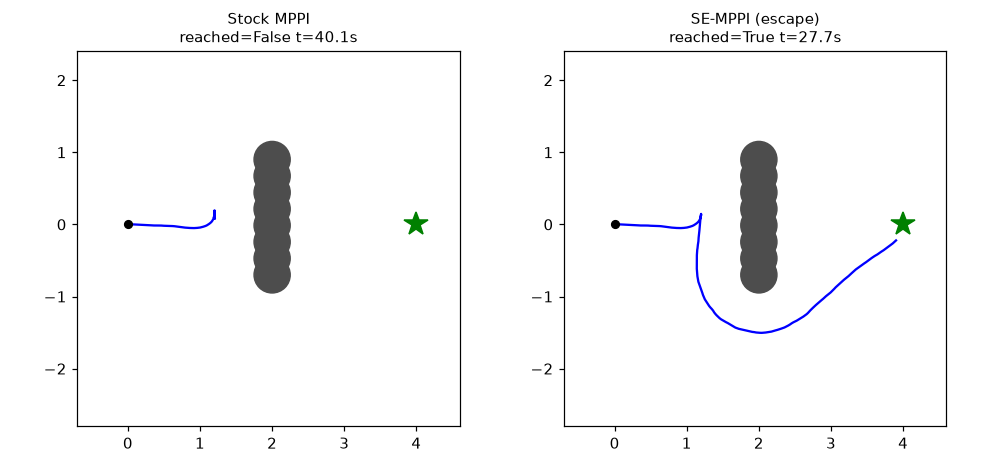
\includegraphics[height=1.55in]{figures/utrap_escape.png}\hfill
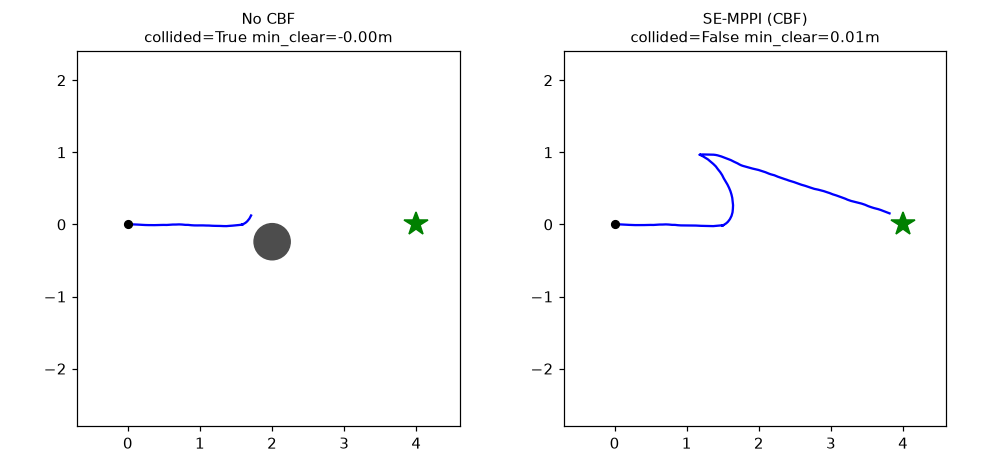
\includegraphics[height=1.55in]{figures/dynamic_cbf.png}\hfill
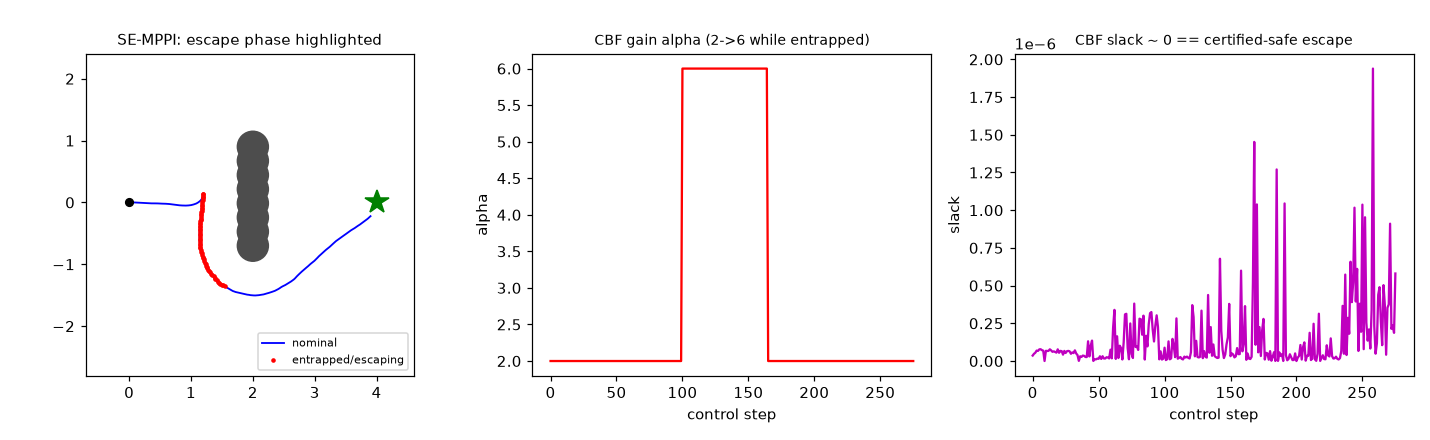
\includegraphics[height=1.55in]{figures/coordination.png}
\caption{Standalone 2D mechanism validation (trajectories/traces only; no
benchmark metrics). \textbf{(a)}~U-trap escape: stock MPPI (left) stalls at
the trap mouth ($x\approx1.2$, no progress) while SE-MPPI (right) detects
the stalled progress and rounds the U-shaped obstacle to the goal via the
gap-attraction subgoal. \textbf{(b)}~Dynamic-obstacle avoidance: against a
crossing obstacle the no-CBF baseline (left) collides while the speed-aware
look-ahead CBF filter (right) projects the command to a collision-free path.
\textbf{(c)}~Escape--safety coordination (the contribution): during the
escape phase the coordinated gain rises $\alpha: 2 \to 6$ while the QP slack
stays $\approx 0$ throughout -- the escape maneuver is admitted yet remains
certified-safe ($h\ge0$), the mechanical evidence for the Proposition of
Sec.~\ref{sec:coordination}.}
\label{fig:mechanism_panels}
\end{figure*}

\subsection{Live Nav2 + Gazebo integration}
\label{sec:integration}

We deployed SE-MPPI in a complete live stack (ROS~2 Jazzy, Nav2 -- AMCL,
costmaps, NavFn, BT navigator, recovery, collision monitor -- and Gazebo
\texttt{tb3\_sandbox}) \cite{nav2} on the target workstation. Confirmed at
the level of committed launch logs and trial telemetry: the controller and
\texttt{EscapeCritic} \textbf{load and activate} from the critics list; the
controller \textbf{produces valid velocity commands} identical in form to
stock MPPI; and the full lifecycle reaches the active state, sustaining
multi-minute drives on a U-trap testbed without a crash or collision after
the ABI fix below (the goal was not reached: the committed telemetry
records STUCK at $254.5$~s and TIMEOUT at $299.8$~s, both collision-free,
under the host constraints noted below). The escape-injection path has also \textbf{run live}: its first live
activation is what exposed the ABI fault below -- a fault unreachable from
unit tests -- and the tensor shapes captured from that event are committed
as a regression test, while the controller and critic now log every
detection and injection transition (\texttt{ENTER}/\texttt{EXIT},
\texttt{BEGIN}/\texttt{END}) for auditability. A sustained live
entrapment-escape demonstration on this host remains confounded by the
host-level artifacts noted below and is deferred to the full-scale
benchmark. We validate the live integration to this depth;
the controlled quantitative comparison is the 2D benchmark of
Sec.~\ref{sec:bench2d}, because a full live A/B on this WSL2 host measures
the host (RTF~$\approx0.3$--$0.6$, with TF smear inflating the costmap with
phantom cells) rather than the algorithm.

Three integration faults surfaced that only a live stack reveals, each
reported as a deployment lesson:
\begin{itemize}
\item \textbf{Static walls in the CBF.} Feeding every lethal cluster
  (including static walls) into the CBF makes the barrier infeasible
  everywhere and freezes the robot -- fixed by scoping the CBF to genuinely
  dynamic obstacles (Sec.~\ref{sec:cbf}).
\item \textbf{Compute budget.} The per-cycle budget must be matched to the
  host (horizon preserved, rate and batch reduced) or the loop misses its
  rate and the optimizer diverges.
\item \textbf{xtensor ABI mismatch.} The installed
  \texttt{libmppi\_controller.so} is compiled with
  \texttt{XTENSOR\_USE\_XSIMD}~+~AVX2 (an \texttt{xsimd::aligned\_allocator}
  element type), whereas our plugin compiled xtensor with the default
  \texttt{std::allocator}. Because \texttt{CriticData}'s tensors cross the
  pluginlib boundary by reference, the first \texttt{EscapeCritic} write to
  \texttt{data.costs} was an ODR violation that segfaulted the entire Nav2
  process on the first live escape injection (3/3 reproducible). The
  in-process unit tests never caught it -- they compile every translation
  unit with one consistent flag set -- and earlier live gates never
  triggered entrapment, so the injection path had never actually run live.
  Fixed by compiling the critic against the installed headers' flags
  (per-target, since a global AVX2 flip breaks the separately built
  OSQP--Eigen boundary); a regression test now replays the injection path
  with live tensor shapes. This is precisely the class of fault a
  Nav2-native deployment exposes and that a standalone node or a pure-2D
  study cannot.
\end{itemize}

\subsection{Randomized 2D quantitative benchmark}
\label{sec:bench2d}

The controlled quantitative comparison is a \textbf{randomized 2D benchmark
that mirrors the controller math one-to-one}. It reuses the exact
primitives validated in Sec.~\ref{sec:mechanism} -- the same MPPI sampler,
distance-field APF, gap raycast, look-ahead CBF-QP via OSQP \cite{osqp},
$\alpha$ coordination with TTC override, and monotone-progress entrapment
detector -- and drives them across \emph{randomized} scenarios so that
success, collision, and clearance carry confidence intervals and paired
significance tests. It is not the live Nav2 controller and inherits the
scope limits of Sec.~\ref{sec:mechanism} (a 2D unicycle, a free-space gap
subgoal in place of global routing, and a look-ahead-\emph{point}
certificate rather than full-body); as in the released controller and the
deployment lesson of Sec.~\ref{sec:integration}, the CBF and TTC see only
the dynamic obstacles, not static walls. We use this 2D surface rather than
a live Gazebo full matrix because at RTF~$0.3$--$0.6$ under CPU contention
the live host measures itself, not the algorithm
(Sec.~\ref{sec:integration}); the full-scale physics benchmark is deferred
to future work (Sec.~\ref{sec:limitations}).

\textbf{Setup.} Four seed-deterministic scenario families exercise the two
weaknesses and their conjunction: \texttt{utrap} (a finite U/C pocket with
the goal behind the back wall -- a static local minimum), \texttt{clutter}
(a random field of 5--9 circular obstacles with a guaranteed
footprint-clear path), \texttt{dynamic} (1--2 pedestrian-like crossing
movers timed to reach the robot's path), and \texttt{narrowdyn} (the
\texttt{utrap} pocket \emph{plus} movers sweeping the pocket mouth during
the escape window -- the narrow-\emph{and}-dynamic coincidence the
coordination targets). Six ablation configs toggle the mechanisms:
\textbf{A}~stock (no escape/CBF), \textbf{C}~escape only, \textbf{D}~CBF
only, \textbf{E}~escape+CBF with
$\alpha_\text{escape}\!=\!\alpha_\text{base}$ (independent), \textbf{F}~full
SE-MPPI ($\alpha\!:\!2\!\to\!6$~+~TTC override, coordinated), and
\textbf{F$^{-}$} (F with the gap search off). Each family is a pure function
of an integer seed, so every config is evaluated on an \emph{identical}
scenario set, as the paired McNemar design requires:
$4~\text{families}\times50~\text{seeds}\times6~\text{configs}=1{,}200$
paired trials, 40~s sim budget each. Success carries a Wilson 95\% CI; the
primary test is McNemar on paired outcomes; continuous metrics use
Mann--Whitney $U$ with Cliff's $\delta$; all $p$-values are
Holm--Bonferroni-corrected within each family.

\begin{table}[t]
\centering
\caption{Randomized 2D benchmark: success rate in \% (Wilson 95\% CI),
$N=50$ per cell. On the trap families (\texttt{utrap}, \texttt{narrowdyn})
the escape configs C, E, F separate from stock~A, CBF-only~D, and no-gap
F$^{-}$; F$^{-}$ collapses to $0\%$; E and F coincide except on narrow-dyn,
where they differ by one trial (64\% vs 62\%).}
\label{tab:bench2d-success}
\footnotesize
\setlength{\tabcolsep}{3.5pt}
\begin{tabular}{lcccc}
\toprule
Config & U-trap & Clutter & Dynamic & Narrow-dyn \\
\midrule
A stock            & 0 [0,7]    & 52 [39,65] & 80 [67,89] & 0 [0,7]    \\
C escape           & 90 [79,96] & 62 [48,74] & 76 [63,86] & 78 [65,87] \\
D CBF              & 0 [0,7]    & 52 [39,65] & 82 [69,90] & 0 [0,7]    \\
E indep.           & 88 [76,94] & 62 [48,74] & 78 [65,87] & 64 [50,76] \\
\textbf{F SE-MPPI} & 88 [76,94] & 62 [48,74] & 78 [65,87] & 62 [48,74] \\
F$^{-}$ no-gap     & 0 [0,7]    & 52 [39,65] & 84 [71,92] & 0 [0,7]    \\
\bottomrule
\end{tabular}
\end{table}

\begin{table}[t]
\centering
\caption{Key paired contrasts (McNemar, Holm-adjusted; $b/c$ discordant
pairs, $b$~= baseline wins, $c$~= F wins). The escape contrast is decisive
on the trap families; the coordination contrast (E$\to$F) is null
everywhere.}
\label{tab:bench2d-stats}
\footnotesize
\setlength{\tabcolsep}{4pt}
\begin{tabular}{lcccc}
\toprule
 & \multicolumn{2}{c}{Escape (stock$\to$F)} & \multicolumn{2}{c}{Coord.\ (E$\to$F)} \\
\cmidrule(lr){2-3}\cmidrule(lr){4-5}
Family & $b/c$ & $p_\text{adj}$ & $b/c$ & $p_\text{adj}$ \\
\midrule
U-trap     & 0/44 & $1.4\!\times\!10^{-9}$\,* & 0/0 & 1 \\
Clutter    & 0/5  & 1                          & 0/0 & 1 \\
Dynamic    & 3/2  & 1                          & 0/0 & 1 \\
Narrow-dyn & 0/31 & $1.1\!\times\!10^{-6}$\,* & 1/0 & 1 \\
\bottomrule
\end{tabular}
\end{table}

\textbf{The escape layer is the measured contribution, and the gap search
is load-bearing.} On both trap families the effect is decisive and survives
Holm correction (Table~\ref{tab:bench2d-stats}): success rises from $0\%$
(stock~A, CBF-only~D, and no-gap~F$^{-}$ all time out in the pocket) to
$88$--$90\%$ on \texttt{utrap} (44/50 discordant pairs, $p_\text{adj}=
1.4\times10^{-9}$) and to $62$--$78\%$ on \texttt{narrowdyn} (31/50
discordant, $p_\text{adj}=1.1\times10^{-6}$). That \textbf{F$^{-}$ scores
$0\%$} on both trap families (Table~\ref{tab:bench2d-success}) shows the
detect-and-switch mechanism escapes only \emph{with} the free-space gap
subgoal: APF and gain modulation without a routed opening do not escape. On
\texttt{clutter} the escape adds $10$~pp ($52\%\!\to\!62\%$, not significant
after Holm) at the cost of $\approx2.4$~s longer average time-to-goal
(over successful trials), and
on the pure-\texttt{dynamic} family -- which contains no trap -- it is
appropriately neutral (Table~\ref{tab:bench2d-stats}, dynamic
stock$\to$F: $p=1$). Fig.~\ref{fig:success_bars} gives the full per-family
picture.

\begin{figure*}[t]
\centering
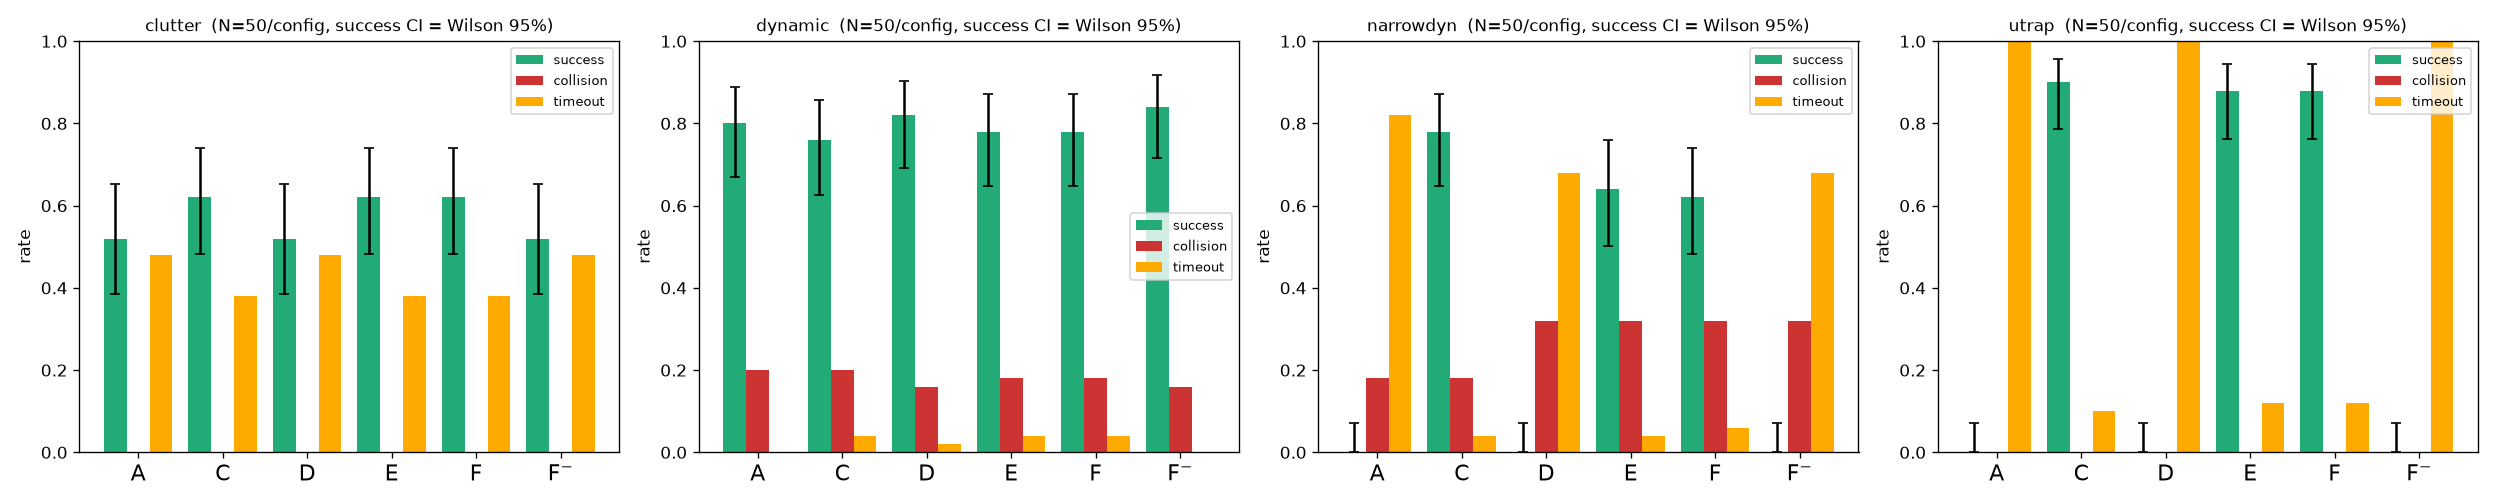
\includegraphics[width=\textwidth]{figures/success_bars.png}
\caption{Randomized 2D benchmark: success / collision / timeout per family
across configs A--F$^{-}$ (Wilson 95\% error bars on success, $N=50$). On
the trap families (\texttt{utrap}, \texttt{narrowdyn}) the escape configs
(C~= escape-only, E~= independent escape+CBF, F~= coordinated) separate
cleanly from stock~A, CBF-only~D, and no-gap~F$^{-}$, which time out at
$0\%$ success. E and F coincide in every family except narrow-dynamic, where
they differ by a single discordant trial (McNemar $p=1$).}
\label{fig:success_bars}
\end{figure*}

\subsubsection{Escape--safety coordination is null in this regime}
\label{sec:evsf}

The load-bearing contrast for the C2 contribution is \textbf{E
(independent) vs.\ F (coordinated)}: identical mechanisms differing only in
whether the CBF gain is coordinated with the escape phase. \emph{Across all
200 paired scenarios this contrast is null} (Table~\ref{tab:bench2d-stats},
Fig.~\ref{fig:e_vs_f}): the discordant counts are $0/0$, $0/0$, $0/0$, and
$1/0$, McNemar $p=1$ in every family, and every continuous effect size is
$|\delta|\le0.03$. The gain does engage as designed
($\alpha_\text{max}=6$ during escape, TTC override active). The committed
per-trial slack telemetry (\texttt{slack\_max} in \texttt{trials.csv};
per-config rates in \texttt{stats.json} and \texttt{tables.md}) locates
where the barrier actually works. On the mover-free families
(\texttt{utrap}, \texttt{clutter}) the dynamic-obstacle CBF sees no
obstacles at all: slack is zero in every trial, E and F issue identical
commands, and the null there is structural. On \texttt{narrowdyn} the
barrier \emph{does} engage and even relaxes -- the QP uses nonzero slack in
$34/50$ trials for E and F ($26/50$ for D and F$^{-}$; max slack $0.47$) --
and on \texttt{dynamic} in $47$--$48/50$ trials (max $0.015$), yet the
E-vs-F contrast stays null ($1/0$ discordant, $p=1$). The correct reading
is therefore not that the barrier never binds, but that \textbf{the
outcomes are insensitive to the $\alpha$ schedule}: where the barrier is
quiescent the two configs coincide exactly, and where it is active the
base and escape gains admit escape maneuvers whose outcomes are
indistinguishable at $N=50$. (The mechanism plot of
Sec.~\ref{sec:mechanism}, ``$\alpha:2\to6$ with slack~$\approx0$,'' shows
the benign end of this spectrum.) We report this honestly: \textbf{in this
2D benchmark the coordination produces no measurable outcome difference
over independent escape+CBF.} The result is consistent with -- and
delimits -- the Proposition of Sec.~\ref{sec:coordination}: coordination
is a \emph{certified-safe mechanism} (the escape maneuver is admitted
while $h\ge0$ is preserved), not, in these scenarios, an outcome
improvement. An outcome-level benefit would require a regime where the
choice of $\alpha$ changes which escape maneuvers are admitted at
outcome-deciding moments -- faster or persistent movers, tighter margins,
a dynamic gap the escape route must thread while the barrier is live;
this generator's pedestrian-like movers produce barrier engagement but
not that sensitivity. Constructing and
measuring that regime is future work (Sec.~\ref{sec:limitations}); we claim
no coordination benefit we have not measured.

\begin{figure*}[t]
\centering
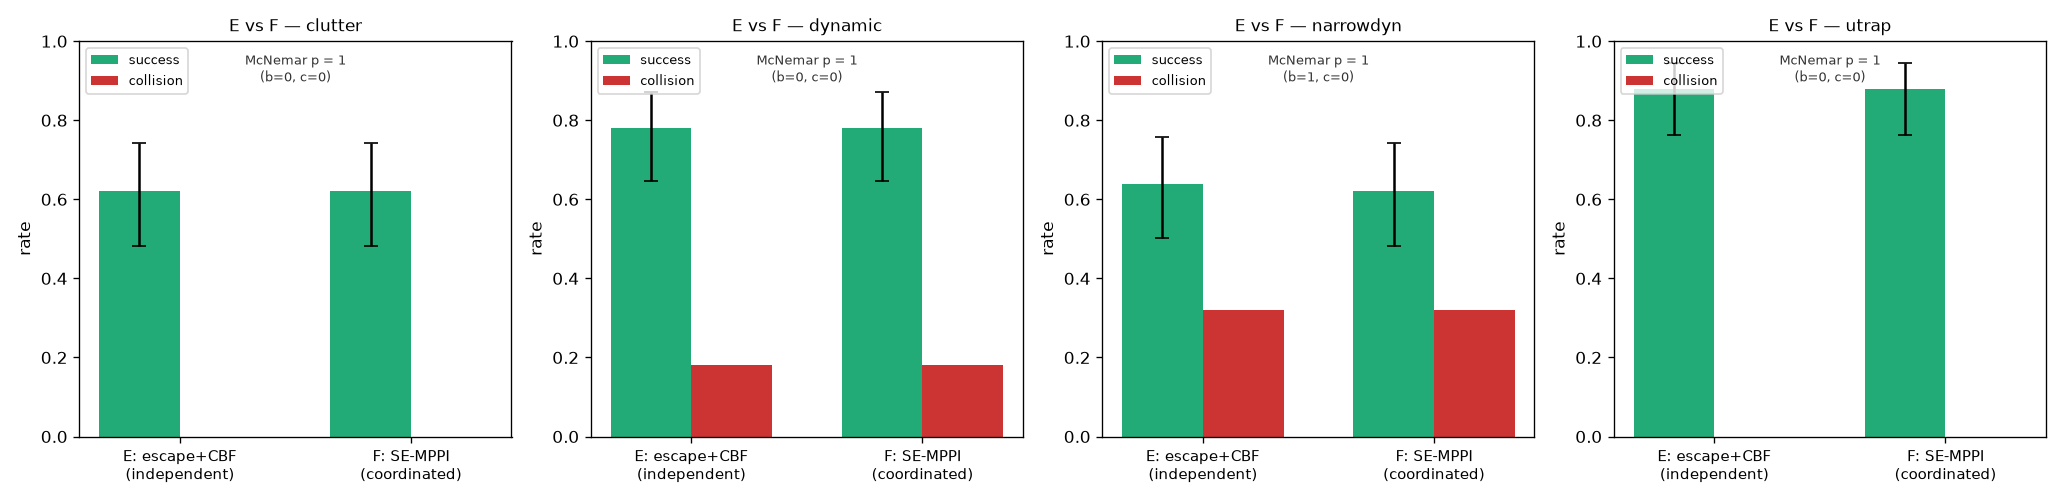
\includegraphics[width=\textwidth]{figures/e_vs_f.png}
\caption{The coordination contrast E vs.\ F per family, annotated with the
McNemar $p$-value. The independent (E) and coordinated (F) stacks are
statistically indistinguishable in every family ($p=1$) -- the null result
of Sec.~\ref{sec:evsf}.}
\label{fig:e_vs_f}
\end{figure*}

Two CBF observations bear on Sec.~\ref{sec:limitations}. Against
body-grazing crossers (\texttt{dynamic}) the look-ahead-point filter
leaves the collision rate essentially unchanged
($20\%\!\to\!16$--$18\%$; descriptive -- the committed analysis carries no
paired collision-outcome test). And in the cramped \texttt{narrowdyn}
pocket the CBF configs show a \emph{higher} collision rate than their
no-CBF counterparts ($18\%\!\to\!32\%$, descriptive) and cost
$\approx16$~pp success ($78\%\!\to\!62\%$; success McNemar F vs.\ C:
$b/c=8/0$, raw $p=0.008$, Holm-adj.\ $0.109$ -- directionally consistent
though not significant after correction at $N=50$). Both are discussed as
limitations in Sec.~\ref{sec:limitations}.

\textbf{Full-scale benchmark (future work).} The live full-matrix
comparison this section stands in for is specified but deferred: an
identical Nav2 stack and differential robot across three tiers -- BARN
(static difficulty) \cite{barn,barn_challenge}, DynaBARN (dynamic)
\cite{dynabarn}, and HuNavSim (human-aware) \cite{hunavsim} -- with stock
MPPI \cite{nav2,mppi_orig}, DWB \cite{dwa}, RPP \cite{rpp}, TEB \cite{teb},
an always-on escape (DRPA-style \cite{drpa_mppi}), and a CBF-only baseline
(Shield-style \cite{shield_mppi}), scored by success, collision,
time-to-goal, path length, clearance, and per-cycle compute under the same
McNemar / Mann--Whitney~+~Holm protocol. Running it on a real-GPU host is
the remaining step (Sec.~\ref{sec:limitations}).

\section{Limitations}
\label{sec:limitations}

\begin{itemize}
\item \textbf{Full-scale physics benchmark is future work.} The
  quantitative comparison in this paper is the randomized 2D benchmark of
  Sec.~\ref{sec:bench2d}, which mirrors the controller math but is not the
  live controller. The full-scale 3D physics benchmark specified there
  (BARN/DynaBARN/HuNavSim against the deployable baselines) is not yet run:
  the live host available to us (WSL2, RTF~$\approx0.3$--$0.6$, with TF smear
  inflating the costmap with phantom cells) measures itself rather than the
  controller (Sec.~\ref{sec:integration}), so it needs a real-GPU host.
\item \textbf{Coordination benefit is unmeasured, not established.} The
  escape--safety coordination (C2) is certified-safe by construction
  (Sec.~\ref{sec:coordination}) but produced no outcome difference over an
  independent escape+CBF stack: outcomes proved insensitive to the
  $\alpha$ schedule even where the barrier engages
  (Sec.~\ref{sec:evsf}). Demonstrating an
  outcome-level benefit requires a regime where the $\alpha$ choice decides
  which escapes are admitted (faster/persistent movers, tighter dynamic
  gaps); constructing and measuring it is future work.
\item \textbf{Braking is not a safe fallback when cornered.} In the cramped
  narrow-dynamic pocket the infeasible-QP fallback ($v=0$) leaves the robot
  in the path of a sweeping mover, and the CBF configs measured a
  \emph{higher} collision rate than their no-CBF counterparts
  ($18\%\!\to\!32\%$; Sec.~\ref{sec:bench2d}). A cornered robot needs an
  evasive fallback, not a stop.
\item \textbf{Look-ahead-point vs.\ full-body safety.} The certificate of
  Sec.~\ref{sec:coordination} is for the look-ahead point $P$ (the
  relative-degree-one output), not the full robot body. Body safety is
  therefore \textbf{approximate}: the offset $L\approx r$ places $P$ at
  the robot's leading edge, and the costmap obstacle critic plus
  \texttt{collision\_monitor} cover the residual. Full-body certification
  would require inflating the margin by $L$, which we deliberately avoid
  because it over-constrains sub-meter gaps (BARN's maximum clearance is
  $\approx 0.9$~m) and would sharply degrade the success rate. This gap is
  measured:
  on the \texttt{dynamic} family the look-ahead filter left body-grazing
  collisions essentially unchanged ($20\%\!\to\!16$--$18\%$, descriptive;
  Sec.~\ref{sec:bench2d}).
\item \textbf{Constant-velocity tracker (addressed in the released
  controller).} The dynamic-obstacle model evaluated in this paper is
  a replaceable constant-velocity (CV) baseline with
  rotating/accelerating agents mispredicted and prediction uncertainty
  unquantified. The released controller now ships (i)~occupancy-persistence
  static/dynamic classification (no wall-freeze on association jitter),
  (ii)~persistent tracks with least-squares CV/CVCA horizon prediction,
  and (iii)~an online conformal bound $q$ that inflates the CBF effective
  radius (time-varying radius) and gates the escape gain on prediction
  trust. The forward-invariance argument is therefore conditional only on
  the \emph{bounded} prediction error that the calibrator maintains, not
  on model correctness. These additions are the subject of the follow-up
  paper (SE-Predict); this paper's claims are isolated from them, and the
  follow-up paper's own no-conformal ablation will isolate them there.
\item \textbf{TTC is a 1-D approximation}; tight spaces can induce
  over-rotation.
\item \textbf{Real-time.} Per-call QP cost grows with the obstacle budget
  (capped by clearance pruning).
\item \textbf{Localization} in symmetric/narrow maps can jump and
  perturb progress estimation -- an environment property, mitigated in
  structured benchmarks.
\end{itemize}

\section{Conclusion}
\label{sec:conclusion}

SE-MPPI packages local-minima escape and control-barrier-function safety,
usually studied apart, in a single deployable Nav2 controller: a shared
entrapment signal drives both a sampling-time escape critic and an
output-time CBF filter, and a coordinated gain lets the robot escape while
a forward-invariance argument keeps the escape certified-safe. A randomized
$1{,}200$-trial 2D benchmark shows the online detection-and-escape layer is
the decisive contribution -- $0\%$ to $88$--$90\%$ success on the static
U-trap family and $0\%$ to $62$--$78\%$ on the narrow-dynamic family, with
the free-space gap search load-bearing -- while the escape--safety
coordination, certified-safe by construction, is empirically
indistinguishable from an independent escape+CBF stack in the regimes we
could test (the null of Sec.~\ref{sec:evsf}), which we report openly. We
fixed three
integration faults that only a live stack reveals -- static-wall CBF
infeasibility, host-matched compute budgeting, and an xtensor ABI mismatch
that segfaulted Nav2 on the first live escape injection -- and confirmed the
controller loads, activates, and runs in a full ROS~2 Jazzy + Nav2 + Gazebo
deployment, with the live injection event that exposed the ABI fault
preserved as a committed regression test. The remaining step is a
full-scale 3D physics benchmark on a real-GPU host. Beyond this paper, the
codebase has grown the
uncertainty-calibrated prediction stack (SE-Predict: classification,
horizons, conformal bounds -- paper 2) and the multi-robot reciprocal
coordination layer (Multi-SE-MPPI -- paper 3); both reuse this paper's
coordination thesis and the shared evaluation harness.

\appendix[Reproducibility]
\label{sec:repro}

All paths below are relative to the code release of contribution C4
(footnote in Sec.~\ref{sec:intro}).

\textbf{Software.} ROS~2 Jazzy, Nav2, and Gazebo are installed via
RoboStack (conda channels \texttt{robostack-jazzy} + \texttt{conda-forge})
by the committed script \texttt{scripts/setup\_ros2\_env.sh}, which also
pulls \texttt{osqp-eigen}/\texttt{eigen} for the CBF-QP \cite{osqp} and the
\texttt{cxx-compiler}/\texttt{cmake}/\texttt{ninja} toolchain, so the build
does not depend on the host OS version (Sec.~\ref{sec:implementation}).

\textbf{Benchmark regeneration.} Every number in Sec.~\ref{sec:bench2d} is
generated from the committed per-trial CSV by committed scripts, never
transcribed by hand. The commands (from
\texttt{docs/papers/2026\_2d-benchmark-results.md}, re-wrapped to column
width; the committed data uses $N{=}50$):

{\scriptsize
\begin{verbatim}
export MAMBA_ROOT_PREFIX=$HOME/micromamba
micromamba run -n ros2 python3 \
  -m experiments.benchmark2d.runner \
  --families utrap clutter dynamic narrowdyn \
  -n <N> --workers 6 --max-steps 400
micromamba run -n ros2 python3 \
  -m experiments.benchmark2d.report  # tables + stats
micromamba run -n ros2 python3 -c \
  "from experiments.benchmark2d import figures, \
aggregate; \
r=aggregate.aggregate( \
  'experiments/results_2d/trials.csv', \
  'experiments/results_2d'); \
figures.plot_all(r['summary'], r['stats'], \
  'experiments/results_2d/figures')"
\end{verbatim}
}

\textbf{Scenarios and seeds.} The benchmark is $4$ families $\times$ $50$
seeds $\times$ $6$ configs $= 1{,}200$ paired trials (seeds $0$--$49$ per
family, $400$ steps $\times$ $0.1$~s budget each). Each scenario is a pure
function of its integer seed: the generators in
\texttt{experiments/benchmark2d/scenarios.py} seed \texttt{numpy}
generators with a deterministic per-family offset plus the trial seed
($10^{6}$ \texttt{utrap}, $2\times10^{6}$ \texttt{clutter},
$3\times10^{6}$ \texttt{dynamic}, $4\times10^{6}$ \texttt{narrowdyn}), and
the MPPI noise stream uses the same trial seed
(\texttt{experiments/benchmark2d/runner.py}), so every config sees
byte-identical worlds and rollout noise -- the common-random-numbers setup
the paired McNemar design requires. The six config toggle sets are
\texttt{experiments/benchmark2d/configs.py}; the ablation overlays for the
deferred live full-scale protocol are
\texttt{experiments/configs/ablations.yaml}.

\textbf{Data and parameters.} Raw per-trial data:
\texttt{experiments/results\_2d/trials.csv}; aggregates and statistics:
\texttt{summary.csv}, \texttt{stats.json}, \texttt{tables.md} (same
directory, all auto-generated). The full released-controller parameter set
is \texttt{src/nav2\_se\_controller/config/}
\texttt{nav2\_se\_controller\_params.yaml}.

% Canonical bibliography lives at docs/papers/references.bib (verified,
% 2026-07-02; see docs/papers/reference-verification-report.md). Referenced
% here via relative path -- tectonic resolves ../references.bib correctly.
\bibliographystyle{IEEEtran}
\bibliography{../references}

\end{document}
